\section{The RAFT Approach}
\label{sec:method}


\subsection{Regulatory Knowledge and Framework Overview}




% To reduce reliance on manual effort in hybrid frameworks, a key challenge is automatically deriving and constructing knowledge to guide intermediate model generation. 
% To this end, we first consider the choice of an appropriate intermediate model. Among various alternatives, we adopt \textit{Formal Requirements}, as they (i) preserve the semantics of natural language rules, and (ii) provide a structured representation suitable for subsequent test generation \cite{gropler2021nlp,yang2025requirements}.

% Given this target, the required knowledge should enable LLMs to generate valid and testable formal requirements. 
% This involves three essential aspects: (i) the fundamental entities involved, (ii) the rules for composing these entities into valid structures, and (iii) the conditions under which formal requirements are testable.
% Accordingly, we define three complementary types of knowledge:
% \begin{enumerate}[leftmargin=*,align=left,label=(\arabic*), itemsep=0pt, parsep=0pt, nosep]
%     \item \textbf{Domain-Specific Meta Model ($\mathcal{M}$)}, which defines the core entities and semantic primitives of formal requirements.
%     \item \textbf{Requirements Representation ($\mathcal{R}$)}, which specifies the symbols, a data dictionary defining their types and value ranges \cite{silberschatz2002database}, and syntactic rules for constructing valid requirements.
%     \item \textbf{Testability Constraints ($\mathcal{T}$)}, which characterize the conditions under which the requirements are considered testable.
% \end{enumerate}
% Together, these components form a unified knowledge system that supports intermediate model generation.
% In the context of compliance testing, we collectively refer to them as \textit{Regulatory Knowledge}.


% Given that LLMs have internalized extensive regulatory knowledge through pretraining, this knowledge remains largely tacit and difficult to leverage \cite{zhang2023large,lu2025tacit}. To bridge this gap, we propose explicating such tacit knowledge into the three explicit artifacts: $\mathcal{M}$, $\mathcal{R}$, and $\mathcal{T}$, and dynamically injecting them into prompt templates to guide LLMs in two tasks: (1) transforming natural language rules into formal requirements, and (2) determining their testability.
% Testable requirements are then used to generate test cases via algorithms.

% In general, we propose \ourtool, a hybrid framework shown in Figure~\ref{fig:framework}, consisting of two phases:


% \textbf{Phase I: Regulatory Knowledge Explication.}
% The meta-model $\mathcal{M}$, requirements representation $\mathcal{R}$, and testability constraints $\mathcal{T}$ are automatically explicated from LLMs, transforming tacit knowledge into explicit and structured artifacts.

% \textbf{Phase II: Prompt and Test Case Generation.}
% The explicated artifacts are dynamically injected into prompt templates to guide requirements generation and testability determination, followed by test case generation, enabling an end-to-end automated workflow.

% The framework is designed to operate in an automated manner by default, while also supporting human-in-the-loop validation when necessary. All intermediate artifacts, such as knowledge artifacts and formal requirements, are stored and can be optionally reviewed and refined in safety-critical or high-assurance settings.


To transform regulations without manual modeling, we use \emph{formal
requirements} that encode domain concepts and behavioral constraints under a
grammar suitable for downstream analysis and generation~\cite{gropler2021nlp,yang2025requirements}.
``Formal'' denotes vocabulary and grammar conformance together with typed,
traceable state and constraint structures for downstream test generation. Each
requirement defines constraints over a pre-operation state, an operation, and
an expected post-operation state, and records its source-rule identifier and
supporting evidence. The downstream generator uses this abstract structure to
derive test cases with inputs, actions, and expected outcomes; an optional
adapter maps their fields to concrete interfaces for automated execution.

The knowledge comprises:
\begin{enumerate}[leftmargin=*,align=left,label=(\arabic*), itemsep=0pt, parsep=0pt, nosep]

\item \textbf{Domain Meta-Model ($\mathcal{M}$):}
the core domain entities and relations used in formalization.

\item \textbf{Requirements Representation ($\mathcal{R}$):}
the symbols, data types, value ranges, syntactic rules, and operational
conventions for constructing and processing valid formal
requirements~\cite{silberschatz2005database}.

\item \textbf{Testability Constraints ($\mathcal{T}$):}
formally stated OCL-style contexts, predicates, and invariants specifying the
conditions under which a formal requirement can be tested. Their semantic
predicates are assessed by LLMs rather than executed by an OCL engine.

\end{enumerate}
Together, they are explicit, reusable \emph{meta-level} artifacts that
operationalize implicit regulatory knowledge in LLMs: what domain concepts are
expressible, how requirements are represented, and what makes them testable.
They do not replace the input regulation, which remains authoritative for
concrete obligations, thresholds, and exceptions. In
Fig.~\ref{fig:framework}, Phase~I elicits LLM parametric
knowledge~\cite{zhang2023large,lu2025tacit}, optionally supported by a
construction corpus. Phase~II injects the resulting artifacts into
current-regulation formalization and test generation.


\subsection{Phase I: Consensus-Based Regulatory Knowledge Explication}
\label{sec:know_ext}


\noindent
\textbf{Initial Attempts and Challenges.}
This phase constructs $\mathcal{M}$, $\mathcal{R}$, and $\mathcal{T}$ from
LLM-generated candidates.
In preliminary trials, the naive prompt ``Construct a financial meta-model for
software compliance testing'' produced relevant entities but unusable
artifacts, exposing two challenges:
\begin{enumerate}[leftmargin=*,align=left,label=(\arabic*), itemsep=0pt, parsep=0pt, nosep]
    \item \textbf{Granularity Inconsistency and Structural Disorganization.} Without explicit constraints, LLMs mix coarse concepts with fine-grained details, yielding disorganized representations that fail to form a coherent hierarchy.
    \item \textbf{Hallucination and Output Variability.} LLMs may produce ungrounded or inconsistent content, and their stochasticity causes substantial cross-run variability, undermining the consistency and integrity
    of the artifacts.
\end{enumerate}

We address them through CoT prompting~\cite{wei2022chain} with optional
retrieval cues and consensus-based \strategy.





\noindent
\textbf{CoT Prompting with Optional Retrieval Cues.}
Because prompt quality is critical for LLM generation~\cite{white2023prompt}, we design a template that integrates CoT reasoning with optional retrieval cues, following established prompt-engineering practice~\cite{chen2025unleashing,sahoo2024systematic}.
It combines four elements: task orientation, optional retrieval cues,
hierarchical decomposition, and granularity constraints, and is applied in
Steps \ding{172}-\ding{174} with task-specific adaptations to generate
$\mathcal{M}$, $\mathcal{R}$, and $\mathcal{T}$.

Without a construction corpus,
the candidates operationally reflect parametric knowledge elicited only by the
domain and task description. With a corpus, both parametric knowledge and
corpus evidence may contribute, and we do not attempt to assign individual
artifact elements causally to either source. Evaluation regulations are unseen
during this phase and remain the authoritative source of rule-level semantics
in Phase~II.


\begin{tcolorbox}[colback=orange!5, colframe=orange!30!black, title=\textbf{Knowledge Explication Prompt Template}, fonttitle=\bfseries\small, fontupper=\footnotesize,
    left=1mm,                       % 左侧内边距
    right=1mm,                      % 右侧内边距
    top=1mm,                        % 顶部内边距
    bottom=1mm,                     % 底部内边距
    boxsep=1mm,                     % 文字到边框的额外间距（可选）
    arc=2mm,                        % 圆角半径（可选）
    rounded corners,                 % 保持圆角
    breakable % 可跨页
]
\sf 
{\small \textbf{\# TASK ORIENTATION}} \\
As a requirements and testing expert, construct \textless a domain meta-model/requirements representation/testability constraints\textgreater\ for \textless financial/road-traffic/power\textgreater\ compliance testing.\\
{\small \textbf{\# OPTIONAL RETRIEVAL CUES}} \\
Use internal domain knowledge to propose reusable meta-level abstractions. When
available, use optional cues as construction evidence for scope, abstraction
granularity, terminology, and output format:\\
- \textbf{Sources:} $\sim$10 domain documents and 10--20 representative tests.\\
- \textbf{Prior artifacts:} $\mathcal{M}$ for $\mathcal{R}$/$\mathcal{T}$; $\mathcal{R}$ for $\mathcal{T}$.\\
Do not treat these examples as substitutes for the regulation formalized in the downstream phase.\\
{\small \textbf{\# HIERARCHICAL DECOMPOSITION}} \\
1. \textbf{Analyze rules:} identify concepts, conditions, actions, and expected outcomes.\\
2. \textbf{Abstract knowledge:} extract structures, semantic relations, domain patterns, and constraints.\\
3. \textbf{Construct the artifact:} organize the knowledge into a coherent, structured, and internally consistent representation.\\
4. \textbf{Review quality:} verify completeness, consistency, semantic correctness, and coherence; refine if needed.\\
{\small \textbf{\# GRANULARITY CONSTRAINT}} \\
Infer scope, granularity, terminology, naming, and format from cues; otherwise use conventional abstractions. Maintain consistency, avoid over/under-specification, and include relevant internal knowledge.
\end{tcolorbox}


\noindent
\textbf{Optional Construction-Corpus Selection and Isolation.}
\ourtool\ can explicate all artifacts without a corpus. The default adds
10 official documents and 20 historical tests per domain as cues for scope,
granularity, terminology, and format; tests span positive, negative, boundary,
and inter-rule cases.

Complete documents are split by source and edition, tests
by source-rule and case identifiers, and cross-partition duplicates are
removed before freezing. Corpus inputs are supplied as complete source-rule and
test-case records rather than vector-indexed overlapping chunks; no embedding
model or vector-retrieval hyperparameter is used. The exact record identifiers
included in each prompt are retained with the run artifacts. The artifacts
never access evaluation documents or labels; held-out rules enter only
Phase~II. Experiment~II evaluates the corpus-free setting.








\noindent
\textbf{\strategy\ Strategy.}
To reduce residual hallucination and variability, \strategy\ consolidates
multi-LLM candidates using an artifact-level policy: purification or
aggregation is assigned by knowledge type, not per element. ``Adaptive''
therefore denotes a high-level policy over the constituent types of regulatory
knowledge as a whole; the type-to-operator mapping is fixed before execution,
not learned or switched at run time.

Before consolidation, candidate names, types, relation endpoints, and grammar
signatures are normalized deterministically. Exact canonical matches merge
directly. For each unresolved pair, GPT-6-Astra~\cite{gpt} receives both
definitions, types or signatures, and, when available, 3--5 supporting rules.
Its constrained output contains an equivalent/non-equivalent decision, a
canonical name, and evidence identifiers. Type-incompatible, unsupported, or
invalid outputs remain distinct. The alignment map and evidence are frozen as
artifact provenance.


For \textit{Domain Meta-Model Construction} (\textit{Step} \ding{172}), the meta-model should follow the principle of structural parsimony, retaining elements that are important and representative~\cite{evans2004domain,harvey2005languages}. The dominant risk here is structural noise from spurious or idiosyncratic elements. We therefore adopt a \textit{$K$-\strategymm} strategy that treats each LLM output as a candidate and retains an element only if it reaches \emph{majority consensus}:


\begin{tcolorbox}[colback=green!5!white, colframe=green!30!black, title={Definition: K-\strategymm}, fonttitle=\bfseries\small, fontupper=\small, rounded corners]
Let $\{\mathcal{M}_i\}_{i=1}^N$ be the meta-models from $N$ LLMs, where each $\mathcal{M}_i=(E_i,L_i)$ consists of entities $E_i$ and relations $L_i$. After semantic alignment of synonymous or equivalent elements, the candidate pools are $\widehat{E}=\bigcup_i E_i$ and $\widehat{L}=\bigcup_i L_i$. Given a strict-majority threshold $K$ ($\lfloor N/2\rfloor+1 \le K \le N$), the purified meta-model $\mathcal{M}=(E,L)$ retains elements supported by at least $K$ LLMs:
\begin{gather}
E = \big\{\, e\in\widehat{E} \ \;\big|\; \textstyle\sum_i \mathbb{I}(e\in E_i)\ge K \,\big\}\\
L = \big\{\, l=(e_a,e_b)\in\widehat{L}\ \ \big|\; \textstyle\sum_i \mathbb{I}(l\in L_i)\ge K,\ e_a,e_b\in E \,\big\}.
\end{gather}
Here, $\mathbb{I}(\cdot)$ is the indicator function. Elements with consensus below $K$ are retained in an auxiliary set $\mathcal{O}=(\widehat{E}\setminus E,\ \widehat{L}\setminus L)$ (``Others'') rather than discarded, preserving potentially useful low-consensus knowledge for subsequent analysis.
\end{tcolorbox}

$N$ and $K$ are configurable; the default $N=3$, $K=2$ follows the
three-backend ensemble and strict-majority rule and is fixed before evaluation.



For \textit{Requirements Representation Formalization} and \textit{Testability Constraints Specification} (\textit{Steps} \ding{173} and \ding{174}), the dominant risk shifts from structural noise to information loss~\cite{zowghi2003interplay}, where a missing symbol, syntactic rule, or testability constraint can directly affect correctness. We therefore adopt an \textit{\strategyrr} strategy that prioritizes logical completeness over frequency:


\begin{tcolorbox}[colback=blue!5!white, colframe=blue!30!black, title={Definition: \strategyrr}, fonttitle=\bfseries\small, fontupper=\small, rounded corners]

Let $\{\mathcal{R}_i\}_{i=1}^N$ and $\{\mathcal{T}_i\}_{i=1}^N$ be the requirements representations and testability constraints derived by $N$ LLMs. After semantic alignment of synonymous or equivalent elements, the aggregated $\mathcal{R}$ and $\mathcal{T}$ are constructed by union, preserving complementary knowledge inferred by different LLMs:

\begin{gather}
    \mathcal{R} = \bigcup\nolimits_{i=1}^N \mathcal{R}_i, \qquad
    \mathcal{T} = \bigcup\nolimits_{i=1}^N \mathcal{T}_i.
\end{gather}
This union-based aggregation retains every aligned symbol, syntactic rule, and testability constraint, without requiring cross-model consensus.
\end{tcolorbox}


Aggregation may retain overlapping grammar productions. Distinct productions
coexist as valid alternatives when each type-checks and parses unambiguously;
their coexistence is not itself a conflict. A deterministic compiler derives
the Xtext \emph{generation view} by merging equivalents, left-factoring
prefixes, checking dictionary types, and enforcing parentheses $>$ comparison
$>$ \textit{AND} $>$ \textit{OR} $>$ \textit{IF--THEN}. Only malformed or
irreducibly ambiguous alternatives are excluded. Requirements that depend on
them are discarded by fully automated \ourtool\ or routed to expert review in
the HITL variant.

Value ranges are defeasible knowledge rather than regulatory authority. If an
artifact range conflicts with the current input regulation, the regulation
overrides it; the source-supported value is used and the conflict is logged in
the requirement provenance.


\begin{figure}[!t]
    \centering
    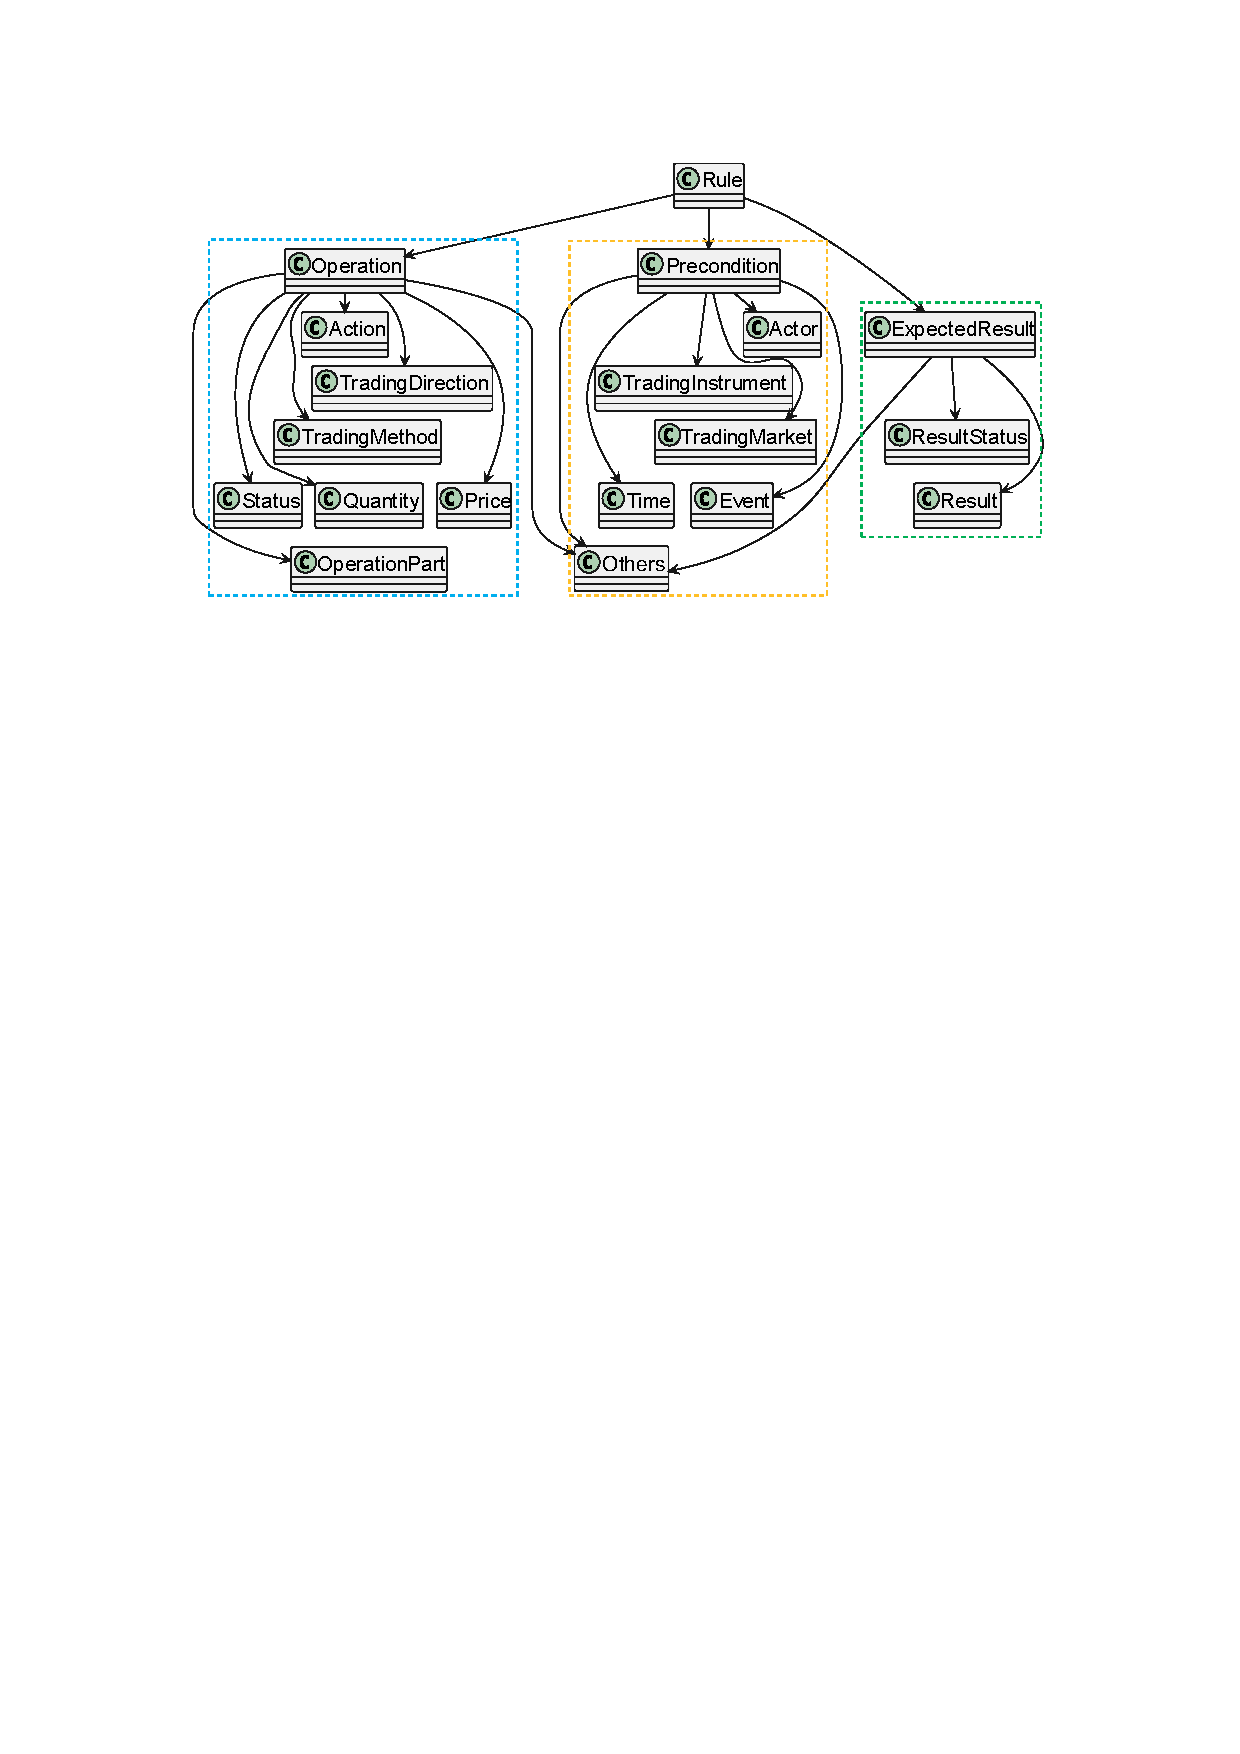
\includegraphics[width=0.7\linewidth]{fig/metamodel_real.pdf}
    \caption{Meta-model for the financial domain.}
    \label{fig:metamodel_real}
    \Description{A hierarchical financial-domain meta-model organizes fourteen entities under precondition, operation, and expected-result categories and shows their relations.}
    \vspace{-2mm}
\end{figure}


\noindent
\textbf{Example of Explicated Regulatory Knowledge.}
We illustrate the artifacts using the default three-LLM ensemble. With 10
regulatory documents, 20 tests, and $N=3$, $K=2$, purification produces
$\mathcal{M}_f$: 14 entities organized under \textit{Precondition},
\textit{Operation}, and \textit{Expected Result} (Fig.~\ref{fig:metamodel_real}).
Fine-grained attributes and values are deferred to $\mathcal{R}_f$.

\begin{figure}[!t]
    \centering
    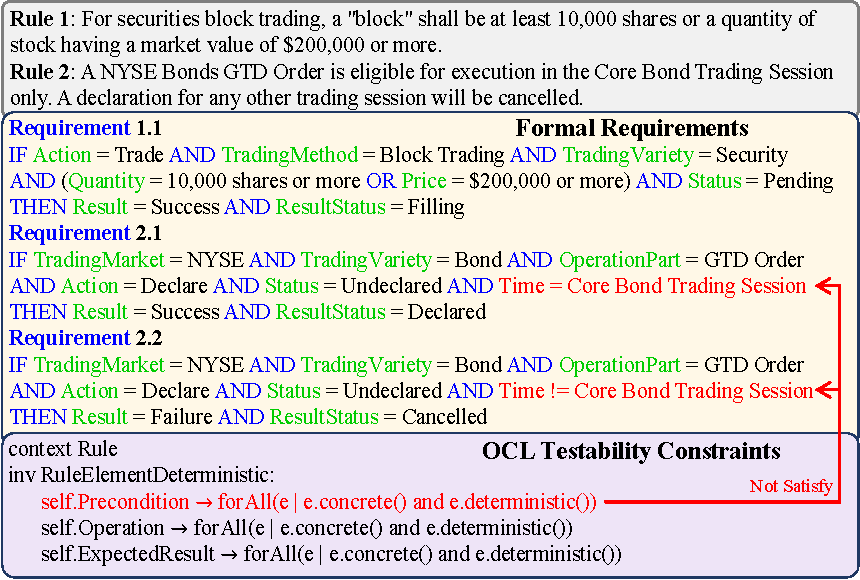
\includegraphics[width=0.7\linewidth]{fig/rule_example.pdf}
    \caption{Two example rules from NYSE~\cite{nyse}, their formal requirements, and their testability decisions.}
    \label{fig:rule_example}
    \Description{Two natural-language NYSE rules are mapped to structured IF-THEN requirements and labeled as testable or untestable according to the five testability dimensions.}
\end{figure}

Each LLM maps $\mathcal{M}_f$ to symbols, a typed data dictionary, and a BNF
syntax~\cite{backus1960report}; aggregation forms $\mathcal{R}_f$ from their
union. Fig.~\ref{fig:rule_example} illustrates its \textit{IF-THEN}
requirements, composed of \textit{KEY-OP-VALUE} expressions joined by
\textit{AND} or \textit{OR}.



Using $\mathcal{R}_f$, the LLMs specify OCL-style constraints~\cite{ocl2014object}
whose union forms $\mathcal{T}_f$. The notation structures LLM assessment but
is not executable OCL. Its five dimensions are structural completeness,
element determinism, action executability, result observability, and rule
non-conflict.
% \begin{enumerate}[leftmargin=*,align=left, itemsep=0pt, parsep=0pt, nosep]
%     \item \textbf{Structural Completeness}, ensuring that the precondition, operation, and expected result are present and not empty.
%     \item \textbf{Element Determinism}, requiring that \textit{KEY} and \textit{VALUE} are deterministic, specific, and free from ambiguity.
%     \item \textbf{Action Executability}, ensuring that operations correspond to concrete actions performable within the system.
%     \item \textbf{Result Observability}, ensuring that expected results are defined and can be objectively measured or verified.
%     \item \textbf{Rule Non-Conflict}, guaranteeing that rules are logically consistent and do not introduce contradictions.
% \end{enumerate}

For example, \textit{Requirement 1.1} in Fig.~\ref{fig:rule_example} satisfies all constraints and is therefore testable, whereas \textit{Requirements 2.1} and \textit{2.2} are deemed untestable because of the non-deterministic expression ``core bond trading session'', which must be concretized as a specific time range (e.g., 9:00--11:30).












\subsection{Phase II: Requirements Formalization and Test Generation}
\label{sec:test_gen}


Phase~II uses knowledge-injected prompting to formalize rules, refine
testability, compose scenarios, and generate implementation-independent tests.


\noindent
\textbf{Knowledge-Injected Prompt Generation.}
In \textit{Step} \ding{175}, two prompts inject the knowledge:

\begin{enumerate}[leftmargin=*,align=left, itemsep=0pt, parsep=0pt, nosep]
    \item $P_\mathcal{R}$ combines $\mathcal{R}$'s schema with task
    decomposition, CoT, and self-critique.
    \item $P_\mathcal{T}$ evaluates each requirement against $\mathcal{T}$ and
    triggers refinement for violations.
\end{enumerate}
$\mathcal{M}$ is not injected directly because it is encoded in $\mathcal{R}$.


\noindent
\textbf{Formal Requirements Generation.}
In \textit{Step} \ding{176}, $P_\mathcal{R}$ adds two workflow annotations:
\textit{Status}, the required pre-operation state, and \textit{ResultStatus},
the expected post-operation state. These annotations define the state boundary
of a requirement and connect otherwise independent requirements into structured
business scenarios when one requirement's post-state satisfies another's
pre-state. They are used only for scenario construction and semantic checking,
not as additional regulatory predicates, and their values must be supported by
the rule or document context.

Our Generate-Verify-Refine loop compiles $\mathcal{R}$'s structured view into
an Xtext syntax validator~\cite{eysholdt2010xtext}. GPT-6-Astra~\cite{gpt}
performs semantic checks: each key must exist in the dictionary, its operator
must be type-compatible, its value must be supported by cited source evidence,
and its state annotations must agree with the operation and outcome. The
checkers return localized diagnostics; refinement changes only flagged
fragments. After three failed repairs, fully automated \ourtool\ discards the
requirement, whereas the HITL variant routes it to expert review. Generated
validators are included in the replication package.




\noindent
\textbf{Testability Determination \& Refinement.}
In \textit{Step} \ding{177}, $P_\mathcal{T}$ uses LLMs to assess each
requirement against every OCL-style predicate by considering the source rule,
document context, structured elements, and logical relationships. The notation
makes each context, predicate, and invariant formally explicit, but predicates
such as determinism and observability require semantic judgment. They are
therefore evaluated by an LLM rather than executed by an OCL engine.

Violations trigger targeted completion or concretization, and the
refined requirement is checked again against $\mathcal{T}$. Every added element
or value must be traceable to the source rule or document context; otherwise,
the requirement remains flagged. Requirements that remain ambiguous, lack
sufficient context, or are inherently untestable are discarded by fully
automated \ourtool\ and routed to expert review only in the HITL variant.





\noindent
\textbf{Scenario \& Test Case Generation.}
In \textit{Step} \ding{178}, testable formal requirements are transformed into
test cases. A requirement precedes another when they concern the same business
object and every canonicalized \textit{ResultStatus} field equals or falls
within the latter's \textit{Status} constraint. Undecidable pairs are not
linked. Chaining these dependencies yields scenario flows; requirements
without state annotations yield only single-rule tests.

Test cases are then generated in two steps. First, Equivalence Partitioning and
Boundary Value Analysis~\cite{graham2006foundations} produce candidate test data
for each constraint. Numerical constraints yield representative valid,
invalid, and boundary values. Finite non-numerical domains are enumerated,
whereas open fields use a satisfying $X$ and a non-satisfying $\neg X$. Second,
these data are assigned to the expression tree encoded by the formal
requirement. The expected validity is the truth value of the complete
expression, evaluated recursively under its operators: conjunction requires
all operands, disjunction requires at least one operand, and implication
$A\Rightarrow B$ is violated only when $A$ is true and $B$ is false. An
assignment with a false antecedent is therefore an antecedent-inactive valid
case, not a violation.

\begin{table}[!t]
    \setlength{\tabcolsep}{8pt}
    \captionsetup{skip=2pt}
    \caption{Selected test cases for \textit{Rule 1} in Fig.~\ref{fig:rule_example}. \textit{Case 4} succeeds because another rule governs that scenario.}
    \label{tab:testcase_example}
    \centering
    \resizebox{\linewidth}{!}{
    \begin{tabular}{|cccccccc|}
    \hline
        \textbf{Test Case} & \textbf{Trading Market} & \textbf{
        Trading Variety} & \textbf{Trading Method} & \textbf{Action} & \textbf{Quantity} & \textbf{Price} & \textbf{Result} \\
        \hline
        \textbf{1} & NYSE & Security & Block Trading & Trade & 50K SH & \$500K & Success \\
        \textbf{2} & NYSE & Security & Block Trading & Trade & 10K SH & \$500K & Success \\
        \textbf{3} & NYSE & Security & Block Trading & Trade & 9K SH & \$100K & Failure \\
        \textbf{4} & NYSE & Security & Auction Trading & Trade & 50K SH & \$500K & Success \\
        \hline
    \end{tabular}
    }
\end{table}


Candidate assignments include active and inactive antecedents. Before pairwise
generation, representative sampling retains one canonical value per
equivalence class; Pairwise Coverage then ensures that each retained value pair
appears in at least one case~\cite{kuhn2004software,myers2004art}. Expected
outcomes and post-states follow the full-expression evaluation
(Table~\ref{tab:testcase_example}). The outputs are compliance test cases with
inputs, actions, expected outcomes, and state transitions.

Each emitted case retains the originating requirement and rule identifiers,
selected equivalence class or boundary value, and full-expression outcome.
This metadata supports audits from each expected result to its source clause
and distinguishes rule-derived values from knowledge-assisted structure; it is
not used as an additional regulatory predicate.


%Pairwise Coverage \cite{kuhn2008automated} is applied, yielding a compact yet comprehensive set of test cases.
%, as exemplified in Table~\ref{tab:testcase_example}.
% We integrate the testable structured requirements into a model-based test case generation workflow. Based on a survey of related work, we adopt LLM4Fin~\cite{xue2024llm4fin}, which is most compatible with our requirement representation. The adapted workflow consists of two stages: Test Scenario Construction, and Test Case Generation.

% Test scenarios are constructed by identifying inter-rule dependencies. Behavioral elements such as \textit{Action} and \textit{Status} are mapped to predefined activity diagrams and state machines, linking individual requirements into end-to-end business flows.

% For each scenario, concrete test cases are derived using diverse test strategies such as Equivalence Partitioning and Boundary Value Analysis \cite{graham2006foundations}. Numerical inputs yield representative positive, negative, and boundary values, while finite non-numerical inputs are exhaustively enumerated. To mitigate combinatorial explosion, Pairwise Coverage \cite{kuhn2008automated} is applied to produce a compact yet comprehensive set of test cases, with an example shown in Table~\ref{tab:testcase_example}.

% Finally, test cases are generated from testable requirements. We apply test strategies such as equivalence class and boundary value analysis \cite{graham2006foundations} to the constraints. Specifically, for numerical constraints, several representative positive, negative, and boundary values are generated. For non-numerical constraints, all values will be enumerated if the value domain is finite; otherwise, only the value itself is used.
% To avoid a combinatorial explosion when multiple constraints interact, we do not perform a full Cartesian product \cite{kuhn2015combinatorial}. Instead, we apply lightweight strategies such as pairwise coverage \cite{kuhn2008automated} and representative sampling. This results in a compact yet comprehensive set of test cases that covers positive, negative, and boundary cases. Table \ref{tab:testcase_example} shows part of the test cases generated for \textit{Rule 1} in Figure \ref{fig:rule_example}.

